\documentclass{article}
\usepackage{maa-monthly}
\usepackage{patrick_custom}
\usepackage{subcaption, tikz-cd}

%% IF YOU HAVE FONTS INSTALLED
%\usepackage{mtpro2}
%\usepackage{mathtime}

\graphicspath{{figures/}}

\theoremstyle{theorem}
\newtheorem{theorem}{Theorem}
 
\theoremstyle{definition}
\newtheorem*{definition}{Definition}
\newtheorem*{remark}{Remark}


\begin{document}

\title{Visualizing Rotations of Space and its Finite Subgroups}
\markright{Rotations and its Finite Subgroups}
\author{}

\maketitle

\begin{abstract}
This paper shows how finite subgroups appear in a natural model of spacial rotations which reflects the geometry of a family of polyhedrons related to a finite rotation group. In particular we emphasize how the symmetries of the Platonic solids contains at least one copy of the object itself, as well as other geometric objects with the same symmetry (sub)group. These copies within the picture correspond exactly to conjugacy classes.
\end{abstract}


\section{Introduction}
    
    The classification of \emph{finite subgroups of spacial rotations}
    \begin{equation}
        \mathrm{FinRot}\coloneqq\curl{G\in \mathrm{Grp}\st G\leq SO(3,\R)\land |G|\in \N}
    \end{equation}
    is well known, we find reference as early as Klein in 1888\cite{klein}. There are two infinite classes:
    \begin{itemize}
        \item $C_k$ - cyclic groups of order $k$ which are the rotations of a $k$-gonal pyramid
        \item $D_{k}$ - dihedral groups of order $2k$ which are the rotations of a $k$-gonal prism
    \end{itemize}
    Exceptionally, the groups $A_4$, $S_4$, and $A_5$ are rotation groups of the regular polyhedrons. Specifically:
    \begin{itemize}
        \item $A_4$ - alternating group on 4 elements, order 12, is the group of rotational symmetries of the tetrahedron, realized as even permutations of its vertices.
        \item $S_4$ - symmetric group on 4 elements, order 24, is the rotational symmetries of the cube, realized as permutations of antipodal pairs of its vertices.
        \item $A_5$ - alternating group on 5 elements, order 60, is the symmetry group of the dodecahedron, by even permutation of five congruent tetrahedral substructures.
    \end{itemize}  This completes the list of finite subgroups of $SO(3)$.
    
    To visualize members of $\mathrm{FinRot}$, we first need a visualization of the space of rotations; that is, we must have a \emph{principle homogeneous space} for $SO(3)$ which is easily inspected.
    \begin{definition}
       A \emph{$G$-torsor} or \emph{principle homogeneous space} for $G$ is a $G$-Set \[(T,-\cdot-:G\times T\to T)\] whose action is free and transitive, that is:
       \begin{equation}
           \forall x,y\in T,\exists! g\in G(y=g\cdot x)
       \end{equation}
    \end{definition}
    Assign to every point $r\coloneqq(x,y,z)^T\in \R^3$ the rotation about the $r$-axis by $|r|$ radians. This is called the \emph{axis-angle} representation. Note that vectors in the same direction that differ in magnitude by $2\pi$ represent the same final state, while also every vectors whose magnitude is an integer multiple of $2\pi$, is a rotation which results in an unchanged final state. Consider the isomorphism of vector spaces defined by
    \begin{gather}
        r=\begin{bmatrix}
        x \\
        y \\
        z \\
        \end{bmatrix}\mapsto x\hat{x}+y\hat{y}+z\hat{z}=:\hat{r}\\
        \text{ where, }\nonumber\\
        \hat{x} = \begin{bmatrix}
        0 & 0 & 0 \\
        0 & 0 & -1 \\
        0 & 1 & 0
        \end{bmatrix},
        \hat{y} = \begin{bmatrix}
        0 & 0 & 1 \\
        0 & 0 & 0 \\
        -1 & 0 & 0
        \end{bmatrix},
        \hat{z} = \begin{bmatrix}
        0 & -1 & 0 \\
        1 & 0 & 0 \\
        0 & 0 & 0
        \end{bmatrix}
    \end{gather}
    so that the hat tracks which algebraic properties of the abstract vector $r\simeq \hat{r}$ are under consideration. This isomorphism grants $\R^3$ the \emph{Lie algebra} structure $\so(3)$, with the multiplication being the \emph{Lie bracket} or \emph{commutator}
    \begin{equation}
        \left[\hat{r}_1,\hat{r}_2\right]\coloneqq\hat{r}_1\hat{r}_2-\hat{r}_2\hat{r}_1
    \end{equation}
    Which is anti-commutative and non-associative; satisfying:
    \begin{gather}
        \left[\hat{r}_1,\left[\hat{r}_2,\hat{r}_3\right]\right]+\left[\hat{r}_2,\left[\hat{r}_3,\hat{r}_1\right]\right]+\left[\hat{r}_3,\left[\hat{r}_1,\hat{r}_2\right]\right]=0\nonumber\\
        \iff\nonumber\\
        \left[\hat{r}_1,\left[\hat{r}_2,\hat{r}_3\right]\right] = \left[\hat{r}_2,\left[\hat{r}_1,\hat{r}_3\right]\right] +\left[\left[\hat{r}_1,\hat{r}_2\right],\hat{r}_3\right]\label{lder}
    \end{gather}
    The Lie algebra $\so(3)$ is the infinitesimal structure of $SO(3)$, vectors $\hat{r}$ are the derivations or \emph{tangent space} at the identity with eqn. \ref{lder} defining the product rule. This completely determines the local structure of the Lie group because this tangent space can be transported to any other by a group element.
    We now get the following
    \begin{definition}[Exponential map]
       The \emph{exponential map} $\exp$ is a smooth map from a \emph{Lie algebra} to its \emph{Lie group} given by the standard power series definition in the matrix algebra over $\R^3$. We are interested in the particular case: 
       \begin{align}
            \exp:\so(3)&\surj SO(3)\\
            \hat{r}&\mapsto \bfr=\sum_{n=0}^\infty\frac{\hat{r}^n}{n!}\nonumber
        \end{align}
        which happens to be surjective and sends $\hat{r}$ to the matrix $\bfr$ for rotation about $r$ by $|r|$ radians by the usual left multiplication action $SO(3)\times \R^3\to \R^3$.
    \end{definition}
    
     For example $\forall\theta\in\R$:
    \begin{equation}
        \exp(\theta\hat{x}) = \begin{bmatrix}
        1 & 0 & 0 \\
        0 & \cos{\theta} & -\sin{\theta} \\
        0 & \sin{\theta} & \cos{\theta}
        \end{bmatrix}.
    \end{equation}
    is a rotation about $(1,0,0)^T$ by $\theta$ radians.
    
    This map is surjective in this instance because $SO(3)$ is compact and connected \cite[Cor. 11.10]{hall}, i.e. \emph{every} rotation is represented in the form $\exp(\hat{r})$ for some $\hat{r}\in \so(3)$.
    Note trivial (identity) rotations by $2\pi$ in any direction are equivalent to doing nothing at all:
    \begin{equation}
        (\hat{0} \sim \hat{r})\iff \hat{r} \in 2\pi\Z S^2\subseteq \so(3)
    \end{equation}
    where $S^2:=\{s\in \R^3\st |s| = 1\}$ is the unit sphere.
    
    Otherwise, non-trivial rotations about the same axis that differ by an integer multiple of $2\pi$ are the same, which defines the equivalence:
    \begin{equation}
       \forall \hat{r}_1, \hat{r}_2\in\so(3)\setminus2\pi\Z S^2 \left((\hat{r}_1\sim \hat{r}_2)\iff\land
       \begin{cases}
       \exists s\in \R&\st\hat{r}_1=s\hat{r}_2\\
       \exists t\in 2\pi\Z&\st|r_1-r_2|=t
       \end{cases}
       \right)
    \end{equation}
    
    This induces the \emph{quotient map}
    \begin{align}
        q: \so(3)&\surj \so(3)/\sim \\
        \hat{r} &\mapsto [\hat{r}] \coloneqq \curl{\hat{r}'\in\so(3)\st \hat{r}'\sim \hat{r}}
    \end{align}
    which is surjective onto the set of equivalence classes named the \emph{quotient space} when equipped with the \emph{quotient topology}: $\Top{q}$. Now we can observe that the axis-angle representation \emph{is} a Lie algebra representative $\hat{r}$ for the preimage $\left[\hat{r}\right]=\exp^{-1}(\bfr)$. Note that $\forall x,y\in \so(3)(x\sim y\iff \exp{x}=\exp{y})$, thus we can utilize the \emph{universal property of quotient maps} to assert the unique existence of the continuous function $\eta$ in the following commutative diagram
    \begin{equation}
        \begin{tikzcd}
        \so(3) \arrow[d, two heads, "q"'] \arrow[rd, two heads, "\exp"] & \\
        \so(3)/\sim \arrow[r, dashed, hook, two heads, "!", "\eta"'] & SO(3)
        \end{tikzcd}
    \end{equation}
    In fact $\eta$ is a \emph{homeomorphism}:
    \begin{itemize}
        \item \emph{injective}\begin{align*}
            \forall&[\hat{x}_1],[\hat{x}_2]\in\so(3)/\sim\\
            [\hat{x}_1]\neq [\hat{x}_2]&\implies \exp(\hat{x}_1)\neq \exp(\hat{x}_2)\\
            &\implies \eta([\hat{x}_1])\neq\eta([\hat{x}_2])
        \end{align*}
        \item \emph{surjective}\begin{align*}
            \forall \mathbf{X}\in SO(3), \exists \hat{x}\in\so(3)\st \exp(\hat{x})=\mathbf{X}\\
            \implies \exists [\hat{x}]\in\so(3)/\sim\st \eta([\hat{x}])=\mathbf{X}
        \end{align*}
        \item \emph{open}---$\forall U\in\tau_{q}, \eta(U) = \exp(q^{-1}(U))\in \Top{SO(3)}$, which is true since $q$ is continuous by property of quotient maps and, in this case, $\exp$ is open\cite[Thm. 2.8]{hall}, as the matrix logarithm is continuous.
    \end{itemize}
    We say that $\exp$ \emph{factors} as $\eta\circ q$. Because $\eta$ is a homeomorphism, the quotient map $q$ is the topological morphology of $\exp$; it captures the mechanics of changing from the topology of $\so(3)\simeq \R^3$ to that of $(\so(3)/\sim)\simeq SO(3)$, an \emph{identification} or \emph{gluing} of points together. The map $\eta$ simply assigns the group structure, as there is none on the quotient space\footnote{The vector addition of $\R^3$ is not everywhere compatible with the equivalence $\sim$ in the standard addition of linearly independent vectors does not preserve the equivalence. However the vector addition is compatible along radial fibers of co-linear vectors individually: $s,t\in\R\implies \exp((s+t)\hat{r})=\exp(s\hat{r})\cdot\exp(t\hat{r})$, and the Lie algebra dictates how the exponential map should glue these fibers together along $\sim$.}.
    
    The gluing $q$ is the central problem of visualization for us. Such a gluing is mechanically impossible in a mere three dimensions, we would need a fourth to bend into to allow such an operation to occur on all radial fibers simultaneously without singular points, or regions of self intersection caused by $SO(3)$'s curvature. However because the space is described in three parameters, we can visualized the un-glued, or \emph{cut} or \emph{flattened} space: the image of a right inverse to $q$, which we shall name $p$.
    
    We define $p$ as the preimage of $q$ intersect a subset of $\so(3)$ such that $p$ is well defined. Consider the open ball of radius $\pi$ in $\so(3)$:
    \begin{equation}
        B\coloneqq\curl{\hat{r}\in\so(3)\st |r|<\pi}
    \end{equation}
    
    $B$ is \emph{almost} an $SO(3)$-torsor; it has unique representatives for all rotations but exact $\pi$ ones. To fix $B$ we give it a ``hat'' $\hem$ of unique $\pi$ rotations. Define
    \begin{equation}
        \hem\coloneqq\curl{\hat{r}\in\partial B\st z>0\lor (z=0\land y>0)\lor x=\pi}
    \end{equation}
    noting that this somewhat arbitrary set has the following critical properties:
    \begin{gather}
        \hat{r}=\pi\frac{\hat{r}}{|r|}\in \hem\implies -\hat{r}=-\pi\frac{\hat{r}}{|r|}\not\in \hem\label{pnp}\\
        \partial B=\hem\sqcup -\hem\label{djb}
    \end{gather}
    Once defining
    \begin{equation}
        \overline{B}\coloneqq B\sqcup \hem,
    \end{equation}
    the function $p$ is a right inverse to $q$ which sends each equivalence class $[\hat{r}]$ to the single element of $[\hat{r}]\cap\overline{B}$. In this way the $\pi$ rotations are assigned to the element that intersects the perfect hemisphere $\hem$, with its critical properties insuring that there exists (by \ref{djb}) a unique (by \ref{pnp}) element $\hat{r}'\in\left[\pi\frac{\hat{r}}{|r|}\right]\cap \hem$:
    \begin{align}
        p:\so(3)/\sim &\inj \so(3) \\
        [\hat{x}]&\overset{!}{\mapsto} \hat{x}'\in [\hat{x}]\cap\overline{B}
    \end{align}
    so that $p$ selects a unique representative for each equivalence class in $\so(3)/\sim$. Note the image is equal to $\overline{B}$, shown in Fig. \ref{fig:log-so3}. \emph{Every figure in this paper is a perspective rendering of $\overline{B}$, usually with some subset of interest highlighted}; as $\overline{B}$ is in bijection with $\so(3)/\sim$, hence is a torsor for $SO(3)$ by the homeomorphism $\eta$. Put another way, this is because the \emph{preimage} or \emph{pullback} $\exp^*$ of a rotation $\bfr$:
    \begin{equation}\label{pimcd}
        \begin{tikzcd}
        \exp^*(\curl{\bfr})\arrow[r, hook] \arrow[d] & \so(3)\arrow[d, "\exp"] \\
        \curl{\bfr}\arrow[r, hook] & SO(3)
        \end{tikzcd}
    \end{equation}
    \begin{figure}
        \centering
        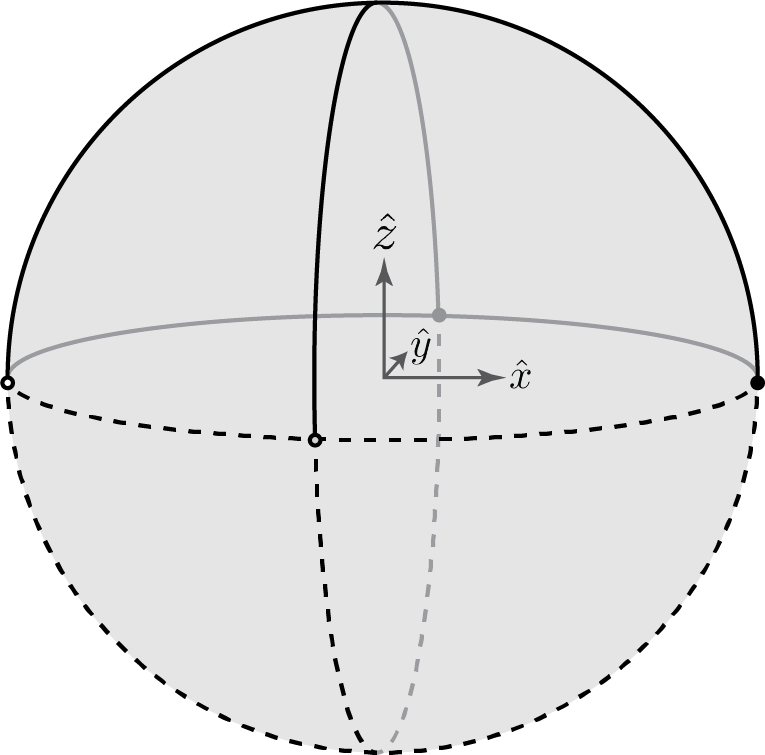
\includegraphics{log-so3-diagram}
        \caption{
        A diagram of $\overline{B}$. The filled and dashed lines indicate where $\overline{B}$ does and does not contain its boundary.
        }
        \label{fig:log-so3}
    \end{figure}
    always intersects $\overline{B}$ exactly once. 
    \begin{definition}[Preimage and Image]
       The \emph{preimage} $f^*$ of a function $f:A\to B$ is a function between power sets $f^*:\pow{B}\to\pow{A}$, satisfying the commutative diagram as in eqn. \ref{pimcd}, that is:
       \begin{equation}\label{def:pim}
           f^*(S)\coloneqq\curl{x\in A\st f(x)\in S\subseteq B}
       \end{equation}
       Following this notation, the \emph{image} $f_*$ is:
       \begin{equation}\label{def:im}
           f_*(S)\coloneqq\curl{f(x)\in B\st x\in S\subseteq A}
       \end{equation}
       so that $f_*:\pow{A}\to\pow{B}$. When there is an identity $\id\in B$, the \emph{kernel} $\ker f\coloneqq f^*(\id)$ is its preimage.
    \end{definition}
    As $2\pi$ rotations are the identity, we get $\ker\exp\coloneqq\exp^*{\id}=2\pi\Z S^2\subset \so(3)$.
    Given $\bfr\neq \id\in SO(3)$ and some $\hat{r}\in\exp^*(\bfr)$, it must be the case that
    \begin{equation}
        \exp^*(\bfr)=\hat{r}+2\pi \Z\frac{\hat{r}}{|r|}\subset \mathfrak{so}(3)
    \end{equation}
    again because $2\pi$ rotations are the identity; co-linear vectors in the Lie algebra that differ in magnitude by an integer multiple of $2\pi$ must map to the same value under the exponential map, and if they do not differ by an integer multiple of $2\pi$, their images must be distinct because there is a non-identity group element $\exp (\hat{r}_1-\hat{r}_2)$ that transforms $\exp \hat{r}_2$ to $\exp\hat{r}_1$ by left multiplication on itself for co-linear vectors $r_1$ and $r_2$. The only relation between non-co-linear vectors are among the elements of $\ker \exp$, or requires consideration of the failure SO(3) to commute, preventing homeomorphism to addition.
    
    Again given some $\bfr\neq\id \in SO(3)$, only one $z\in \Z$ gives a point in the half closed ball, $\overline{B}$, since its diameter is $2\pi$ and it contains at most one of any given pair of antipodal points. We can define $\log$:
    \begin{align}
        \log: SO(3)&\inj \so(3) \\
        \bfr&\mapsto \hat{r}\in\exp^*(\bfr)\cap \overline{B} = p\circ \eta^{-1}(\bfr)
    \end{align}
    %Therefor $B/\sim$ is a \emph{principal homogeneous space} for $SO(3)$. (didn't actually use the def of PHS, perhaps alter this) I name the unique element $\log(\bfr)\coloneqq\exp^{-1}(\bfr) \cap \overline{B}$. The gluing insures $\exp\circ\eta^{-1}$ is indeed a homeomorphism, essentially, $\exp$ re-glues what $\eta^{-1}$ \emph{cuts}. Cuts are the opposite of a gluing, in that $\eta$ being a gluing means $\eta^{-1}$ is a cut. This paper is concerned with visualization, and I can only draw subsets of $\R^3$. 
    Every diagram depicts $\log_*(G)\subset\overline{B}=\log_*(SO(3))\subset\so(3)$ where $G\in \mathrm{FinRot}$, i.e. every visualization is a \emph{cut} view of $SO(3)$, because $\log$ is left inverse to the gluing $\exp$:
    \begin{equation}
        \begin{tikzcd}
           & SO(3)\arrow[dr, hook, "\log"] & \\
           \so(3) \arrow[ur, two heads, "\exp"]\arrow[rr, "\id"]&& \so(3)
        \end{tikzcd}
    \end{equation}
    We focus on $\overline{B}$ because it is an $SO(3)$-torsor under the action (check this!)
    \begin{align}
        SO(3)\times \so(3)&\to \so(3)\\
        (\G,\hat{x})&\mapsto \log(\G\exp{\hat{x}})\nonumber
    \end{align}
    
    Earlier we called the image of $G$ under $\log$ that subgroups' ``flattening''. We chose this name as an metaphor based on how the exponential map works for pure imaginary numbers: a bijection exists between the unit circle and any length $2\pi$ contiguous line segment of pure imaginary numbers containing a single boundary point, for example $\curl{ix\in\C \st x\in(-\pi,\pi]\subset\R}$. Because this set contains "half" its boundary, we will call it half closed. Identifying the boundary points of this segment ($i\pi\sim -i\pi$) forms a ``flat circle'', the identification captures the topological properties lost by cutting the circle into a segment. We essentially did this same process in higher dimensions with every great circle through the identity in $SO(3,\R)$ flattened into $2\pi$ length segments along axes centered on 0 in $\overline{B}$. By identifying antipodal boundary points we make a ``flat $SO(3,\R)$'' called $B/\sim$, and the set $\overline{B}$ as the image of $p$ is our method of inspecting this flat $SO(3)$.
    
    For finite subgroups, the placement of group element representatives in our drawings is restricted by order:
    \begin{theorem}\label{thm:sphereclass}
        If an element $\G\in G\leq SO(3)$ has order $\left|\G\right|=n\in\N$, then its representative $\hat{g}=\log(\G)\in \overline{B}$ must lie in a sphere of radius $|g|=2\pi k/n$ where 
        \begin{equation*}
            (2k\leq n)\land (k|n\implies k=1).
        \end{equation*}
    \end{theorem}
    \begin{proof}
    By assumption:
    \begin{equation}
        \id = \G^n = \exp(n\hat{g})
    \end{equation}
    The equivalence $\sim$, i.e. that rotations by $2\pi$ are the identity, implies there is a $k\in\Z$ where
    \begin{equation}
        n\hat{g}=2\pi k\frac{\hat{g}}{|g|}\implies |g|=\frac{2\pi k}{n}
    \end{equation}
    while $\hat{g}\in \overline{B}$ so $2\pi k/n\leq \pi$ hence $2k\leq n$. Suppose $k|n$, then
    \begin{gather}
        \exp(\hat{g}n/k)=\exp(2\pi \hat{g}/|g|)=\id\\
        \implies\G^{n/k}=\G^n=\id
    \end{gather} and $n$ is the smallest integer where $\G^n=\id$, hence $k = 1$.
    \end{proof}
    Furthermore, for every $k\in \N$ satisfying the above, there is an element
        \begin{equation*}
            \G^k=\exp\left(\frac{k}{n}\frac{2\pi \hat{g}}{\left|g\right|}\right)\in G
        \end{equation*}
    which also has order $n$, as can be seen by the non-divisibility condition $k|n\implies k=1$.
    This theorem restricts the placement of representatives in $\overline{B}$ to concentric spheres centered at the origin of radius $2\pi k/n$ for symmetries of order $n$. This together with the geometry of objects related to a given rotational symmetry $G$ allows us to place all group element representatives of $\log_*(G)\subseteq \overline{B}$ without direct calculation. These geometric objects are the conjugacy classes of the group realized as the 0-skeleton, a set of point suspending a regular 2-cell complex homeomorphic to the sphere or \emph{polyhedron} within $\R^3$.
    
\section{Derived Polyhedra}

We follow inspiration from Hatcher \cite{MR1867354} in notation, defining a point or \emph{0-cell}, and inductively define  the unit open $n$-disk or \emph{$n$-cell} as
\begin{gather}
    e^0\coloneqq \star\\
    e^n\coloneqq \curl{(x,y)\in \R\times e^{n-1}\subseteq \R^n\st x^2+||y||^2<1}
\end{gather}
so that the upper index tracks cell dimension.
Take as given a polyhedron $P$ realized as a flat celled, finite \emph{2-CW complex} embedded in $\R^3$ and homeomorphic to the sphere, equipped with the largest group $\rot{P} \coloneqq G\leq SO(3)$ that has a free action $\alpha$ on $P$, called the \emph{rotations of $P$}: 
\begin{align}
    \alpha:G\times P&\to P\\
    (\G,x)&\mapsto \G\cdot x\nonumber
\end{align}
\begin{definition}[Regularity]
    We call $n=|\rot{P}|$ the \emph{regularity} of polyhedron $P$. Thus polyhedrons with large free group actions are \emph{regular}.
\end{definition}
\begin{definition}[Adjacent cells and shells]
    A pair of cells $e^i_a, e^j_b\in P$ are adjacent $e^i_a ||| e^j_b$ if either is part of the boundary of the other.
    \begin{equation}
        e^i_a ||| e^j_b \defeq e^i_a \subset \partial e^j_b || e^j_b\subset\partial e^i_a
    \end{equation}
    The set of cells adjacent to a given cell is its shell.
    \begin{equation}
        \shell{e^i_a}\coloneqq \{e^j_b\in P\st e^i_a|||e^j_b\}
    \end{equation}
\end{definition}
As a CW complex, $P$ is a disjoint union $P^0\sqcup P^1\sqcup P^2$, called a \emph{cellulation}, of its:
\begin{itemize}
    \item vertices named $P^0$ (0-cells). Formally a $J$ finitely indexed family of maps from the singleton $P^0\coloneqq\curl{e^0_j:e^0\to \R^3}_{j\in J}$ with all distinct images $(i\neq j\implies e^0_i\neq e^0_j)$. The orbit of a vertex must stay a constant distance from the origin because $G$ is a subgroup of $SO(3)$. This means that if the rotations are transitive on vertices, then the vertices $P^0$ are inscribed in a sphere.
    \item edges named $P^1$ (1-cells). A family of continuous maps $P^1\coloneqq\curl{e^1_{ij}: e^1\to \R^3}_{(i,j)\in K}$ indexed by a subset $K\subseteq J\times J=J^2$ so that $(i,j)\in K$ implies $e^0_i$ and $e^0_j$ have no closer co-planar through the origin neighbors (
    \begin{equation}
        |e^0_i-e^0_j|=\min \curl{|e^0_{i'}-e^0_{j'}|}_{(i',j')\in J^2}
    \end{equation}
    We use segments, defined as functions of $t\in e^1$, satisfying:
    \begin{equation}
        e^1_{ij}(t)\coloneqq\frac{(t+1)e^0_j-(t-1)e^0_i}{2}
    \end{equation}
    so that $\partial e^1_{ij}=\curl{e^0_i, e^0_j}$; they are flat (straight) segments suspended between pairs of adjacent 0-cells.
     
    A general 1-cell may loop from a vertex to itself, however for a polyhedron defined this way every edge terminates in two distinct points, the boundary $\partial e^1_{ij}$.
    \item  faces named $P^2$ (2-cells). A family of continuous maps $P^2\coloneqq\curl{e^2_{\Delta}: e^2\to \R^3}$ indexed by loops of edges $\Delta$, so that $\partial e^2_{\Delta}=\Delta$. 
\end{itemize}

A (possibly non-distinct) co-planar loop can be assigned to every 1-subcomplex of the form
\begin{gather*}
    e^1_{ijk}\coloneqq\curl{e^0_i,e^1_{ij}, e^0_j, e^1_{jk}, e^0_k}\\
    \st \paren{\sum_{\ell\in \curl{i,j,k}}\lambda_\ell e^0_\ell = 0\implies \lambda_\ell = 0}
\end{gather*}
a path with 3 linearly independent yet $e^0_j$ adjacent vertices, as $\Delta\coloneqq\partial\paren{P\cap e^2_{ijk}}=e^1_{jk\dots ij}: S^1\simeq\partial e^2\hookrightarrow \R^3$ where $e^2_{ijk}$ is the plane spanning the 3 points $\curl{e^0_i,e^0_j,e^0_k}$, unique because the points are restricted to a sphere and hence always not co-linear. For reasons we will see, this loop may consist of 3 to 5 edges/vertices: triangles, squares and pentagons, except for dihedral/cyclic regular polyhedrons, which have 1-2 faces with any number or edges and vertices. The singular 2-subcomplex  $e^2_{\Delta}$ maps the unit open disc to the interior of the polygon bounded by $\Delta$ in this plane.
In this way the polyhedron has some nice algebraic properties:
\begin{gather}
    \partial P^d = \bigsqcup_{c<d}P^c\label{pbd}\\
    G\cdot P^d\coloneqq\curl{g\cdot x\in P\st (g,x)\in G\times P^d}=P^d\label{cinv}\\
    \sum_{d=0}^2(-1)^d|P^d|=2\label{eucha}
\end{gather}
 Property \ref{pbd} is by definition for constructing a finite cell complex. Property \ref{cinv} states that the group must independently stabilize each cell type. Finally property \ref{eucha} is the Euler characteristic formula for 2-CW complexes homeomorphic to the sphere.
%  This immediately gives a collection of associated homomorphisms for every $i\in\curl{0,1,2}$:
%  \begin{gather}
%      \phi_{i}:G\to S_{|P^i|}
%  \end{gather}
%  by tracking the group action on the $P^i$ separately.

 There are several polyhedra that are invariant under the same group action generated by replacing related $d$-cells with their centroid $0$-cells, then generating a new polyhedron from these vertices as above. The obvious case is when $P$ is regular and has the dual polyhedron generated by assigning every 2-cell of $P^2$ its centroid to get a derived set of 0-cells, which has associated faces and edges, which in this case happen to be in bijective correspondence with $P^0$ and $P^1$ respectively, the other components of the complete dual polyhedron $DP^2$.
 
 \begin{definition}[Similar cells]
    We say a pair of cells $A, B\subseteq P^n$ are \emph{similar} if there exists a $\G\in G$ such that $A=\G\cdot B\coloneqq\curl{\G\cdot b\st b\in B}$ as sets.
 \end{definition}
 \begin{theorem}[Similar cells have similar shells]
     If $A, B\subseteq P^n$ are similar cells, then the shells $\shell{A}, \shell{B}$ of each must be composed of 1-1 corresponding similar cells. This is because the $\G$ action works on the whole polyhedron and preserves boundary relation.
     \begin{gather}
         \G\cdot A= B\implies \G\cdot \partial A = \partial B\\
         \G\cdot \shell{A} = \{\G\cdot A'|||\G\cdot A = B|A'|||A\} = \shell{B}
     \end{gather}
    
 \end{theorem}
 For polyhedrons:
 The shell of a 0-cell is always an alternating ``petals'' of 2-cells and their 1-cell boundaries. The shell of a 1-cell is always a pair each of 0-cells (the boundary of the 1-cell) and 2-cells (whose boundary contains the 1-cell). The shell of a 2-cell is just its boundary composed of alternating 0 and 1-cells.

 Most regular polyhedra symmetries are transitive on vertices so all 0-cells are similar. However most dihedral diamonds have a pair of antipodal points non-similar to the bulk other perimeter points -- the rare exception only the (regular) 4-dihedral diamond corresponding to a regular octohedron as $<(123)>\rtimes <(13), (1234)> = S_4$. The normal subgroup of 3 cycle symmetry of the regular octohedron $\implies$ equilateral triangular faces.
 
 In general not all 2-cells $P^2$ of $P$ are similar, i.e. they do not have the same topological shape in the sense of how many 0-cells and 1-cells compose its boundary. If a pair of 2-cells $A,B\in P^2$ do not have the same number and type of subcells on their boundary then no symmetry $g\in G$ could map $A=g\cdot B$ because such a map must map cells of the same dimension to each other to maintain compatibility of the group action with the cell topology, and thus cannot form the required bijection between subcells on the boundaries when the number of subcells differs.
 However $P$ is regular if and only if every 2-cell is similar (check this).
 \begin{definition}[Derived polyhedron]
    A \emph{derived polyhedron} is generated by placing a vertex at the centroid of each similar singular subcomplex of $P$, then generating a new polyhedron inductively from these vertices as
 \end{definition}
 
 Consider the collection of all subcomplexes
 \begin{equation}\label{def:subc}
     \subc{P}\coloneqq\curl{C\subseteq P:C\text{ is a closed cell complex}}
 \end{equation}
We can partition the collection of subcomplexes 
\begin{equation}
    \subc{P}=\bigsqcup_{s\in S}\Orb_s
\end{equation}
 by similarity $S$, as orbits $\Orb_s\coloneqq G\cdot C_s$ of the \emph{pushforward} of $\alpha$:
 \begin{align}
     \alpha_*:G\times\subc{P}&\to \subc{P}\\
     (\G, C)&\mapsto \G\cdot C\nonumber\\
     \text{where, } G\cdot C\coloneqq \curl{\G\cdot x\in P\st(\G, x)\in G\times C}\nonumber
 \end{align}
 Is the action induced by all of the inclusions of subcomplexes $C$ into $P$. We interpret these orbits as similarity classes of shapes, where by shape we mean a particular arrangement of cells in a subcomplex invariant under the action of its stabilizer. The stabilizer subgroup acting on the subcomplex determines how the cells of its boundary can be arranged because the ambient group action independently stabilizes cells by dimension and the dimension of the boundary must be distinct (one less) from the whole set. Similar subcomplexes thus have the same shape because their stabilizers are conjugate and hence isomorphic.
 
 Of particular interest to us are the similarity or \emph{shape} classes $\Orb^d_s\coloneqq G\cdot C^d_s\in \subc{P^d}/G$ of the various singular $d$-cell complexes $C^d_s\coloneqq e^d_s\sqcup \partial e^d_s$ about some single $d$-cell $e^d_s\in P^d$ with shape $s\in S$; as there may be multiple shapes for fixed cell dimension.
 However $d=2$ is the first case where one singular $d$-cell may not be similar to another. In particular:
 \begin{itemize}
     \item $d=0$, then the boundary $\partial e^0_j$ is empty, and every pair of singular $0$-cell with similar shells are similar.
     \item $d=1$, then the boundary $\partial e^1_{ij}$ is the pair $\curl{e^0_i, e^0_j}$ and so every singular $1$-cell in a polyhedron is similar to a subcomplex homeomorphic to the closed interval, so that its stabilizer is isomorphic to a subgroup of the group of order $2$ acting by $t\mapsto -t$ in $e^1_{ij}$ and $e^0_i\mapsto e^0_j$ on its boundary.
     \item $d=2\implies \partial e^2_n=\Delta_n$ where $\Delta_n=e^1_{jk\dots ij}$ and $jk\dots ij$ has length $n$ and specifies a loop 1-subcomplex with $n$ edges suspended sequentially between $n$ linearly independent vertices based at $e^0_j$.
 \end{itemize}
 
%  Given some $d$-cell $S\in P^d$, assign $S$ its \emph{stabilizer} $G_S$, the subgroup of $G$ fixing $S$, and note that similar subcomplexes have conjugate stabilizers and vice versa.
%  \begin{align*}
%      A=g\cdot B\iff G_A &= G_{g\cdot B}\\
%      &=\curl{h\in G:g\cdot B = hg\cdot B}\\
%      &=\curl{h\in G: B = g^{-1}hg\cdot B}\\
%      &=\curl{h\in G:g^{-1}hg\in G_B}\\
%      &=gG_Bg^{-1}
%  \end{align*}
 
We analyze the partition into $\bigsqcup_{s\in S}\Orb^d_s$ by considering the action of the \emph{stabilizer} $G^d_s$ of some $C^d_s$ on its boundary subcomplex, where the first non-trivial case being $d=2$: 
\begin{align}
    \partial C^2_s=\bigsqcup_{e^0_j\in \partial C^d_s}e^0_j\sqcup\bigsqcup_{e^1_{ij}\subseteq\partial C^d_s}e^1_{ij}
\end{align}
The \emph{orbit-stabilizer theorem} tells us that:
\begin{equation}
    |\Orb^d_i|=\left[G:G^d_i\right]
\end{equation}
so that in particular the number of similar subcells within $P$ must divide the order of $G$.
 
A derived polyhedron $D_i P^d$ exists for each orbit $\Orb^d_i$ in $\subc{P^d}/G$ whose $|\Orb^d_i|$ vertices are given by the centroids of $i$-cells in $\Orb^d_i$.
 
The dual of a regular polyhedron above is one type of derived polyhedron. Because every 1-cell of $P$ is similar, since each is an open interval bounded by a pair of distinct vertices hence stabilized by a subgroup isomorphic to $S_2\simeq C_2$; there is another kind of derived polyhedron given by assigning to every 1-cell of $P$ its centroid 0-cell, written $DP^1$.
 
An interesting question for further research is: how does this process generalizes to higher dimensions?
 
\section{Cyclic and Dihedral groups}

\begin{figure}
    \centering
    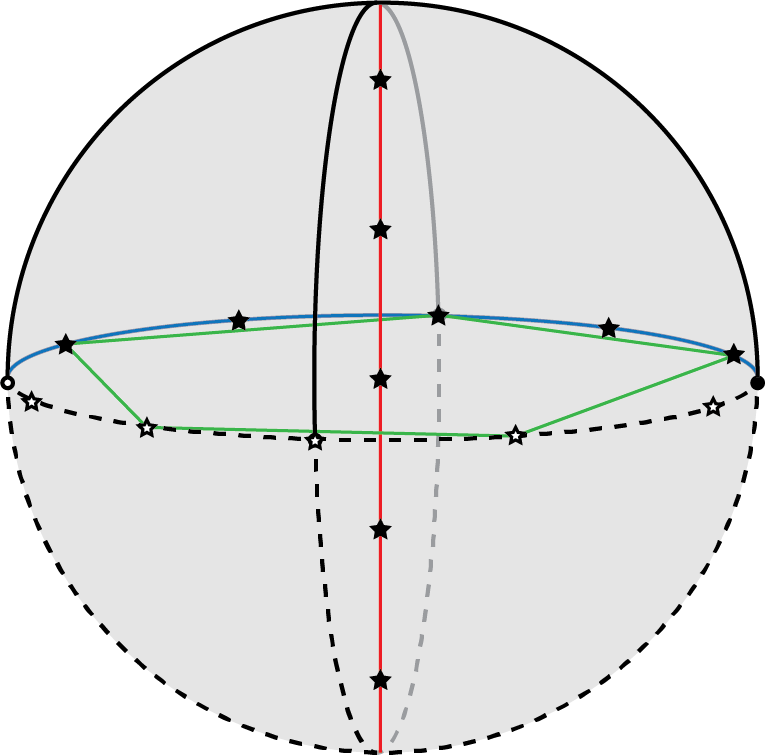
\includegraphics{d5-in-so3}
    \caption{$D_5\leq SO(3,\R)$ illustrated in $\overline{B}$}
    \label{fig:D5inSO3}
    \caption{Unfilled stars are the same point as opposite filled stars on the blue pentagonal circle under the $2\pi$ difference identity}
\end{figure}

$C_k$ is a subgroup of $D_k$, so we will restrict our visualization to the latter; the former is just a subset of the diagram. Consider $D_5$, the symmetries of the regular pentagon. Without loss of generality we assume the pentagon in question is centered at the origin with a vertex on the positive $y$-axis, for example the green pentagon shown in figure \ref{fig:D5inSO3}. The class equation is $|D_5|=1+2+2+5$.

In this diagram (Fig. \ref{fig:D5inSO3}), the stars are the group elements. The subgroup $C_5$ of rotations about the $z$-axis are the stars along the vertical red line. The coset of that subgroup, all of the ``flips'' sending $\hat{z}\to-\hat{z}$, are the stars along the blue line. Note that every group element of order 2 lies in $\partial B$; this is the first example of our usage of Thm. \ref{thm:sphereclass}: every element of order 2 must lay in a sphere of radius $\pi$ since $k=1$ is the only possibility when $n=2$. The unfilled stars show where the other members of the equivalence class defined by $\sim$ are located on $\partial{B}$, and help emphasize how the conjugacy class with 5 group elements, \emph{the 2-cycles, are a pentagon} (green). Of course the fact that groups act on themselves helps justify why this should be the case. In particular the adjoint action of a group on itself fixes the conjugacy classes, and we see $D_5$ has such a class that is also a pentagon.

In fact there is another pentagon in this picture, although it is obscured by our flattening of $SO(3)$, the five stars on the red line, which contain the \emph{5-cycles}. Since $n=5$, $k=1,2$ are the two possibilities, the 4 elements of the 5-cycles lie at the 4 intersection points of the $\hat{z}$-axis and the two spheres of radius $r=2\pi/5, 4\pi/5$. These are the 2 conjugacy classes with 2 elements each. The 5-cycles together with the identity form the subgroup $C_5$.

The blue and red line are a pair of interlinked \emph{great circles}, and the stars are equally spaced on these circles, \emph{making $D_5$ a pair of interlinked regular pentagons embedded in $SO(3)$}.

I only show this one example and leave the reader to consider how other dihedral groups (and cyclic subgroups) would appear in this diagram scheme. What changes when the dihedral group is over an even rather then odd number, like $D_6$?
\section{Alternating and Symmetric groups}
$A_4$ is a subgroup of $S_4$ so again we move to discuss the latter. It is the rotational symmetries of the dual objects hexahedron (cube) and octohedron both, as well as one Archimedian solid, the cuboctahedron. The class equation is $1+6+8+6+3 = 4!$, and since it is a full symmetric group cycle type determines conjugacy class. The cycle type also determines the order of an element, so Thm. \ref{thm:sphereclass} again restricts placement.

\begin{figure}[h]
    \begin{subfigure}{.49\linewidth}
    \centering
    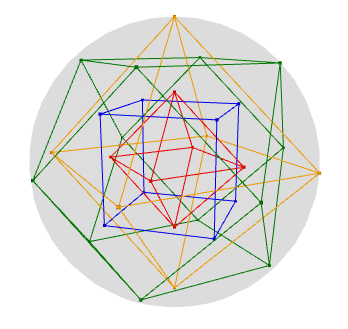
\includegraphics[width = \linewidth]{s4}
    \caption{$S_4$ illustrated in $\overline{B}$}
    \end{subfigure}
    \begin{subfigure}{.49\linewidth}
    \centering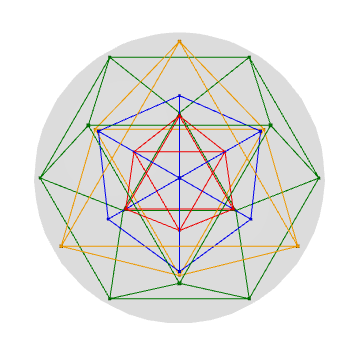
\includegraphics[width=\linewidth]{s4-3cycle}
    \caption{viewed along a 3-cycle axis}
    \end{subfigure}
    \begin{subfigure}{.49\linewidth}
    \centering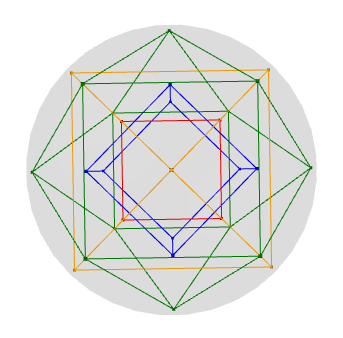
\includegraphics[width=\linewidth]{s4-4cycle}
    \caption{viewed along a 4-cycle axis}
    \end{subfigure}
    \begin{subfigure}{.49\linewidth}
    \centering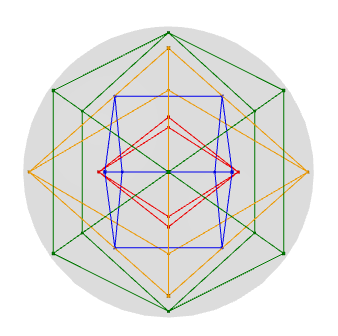
\includegraphics[width=\linewidth]{s4-2cycle}
    \caption{viewed along a 2-cycle axis}
    \end{subfigure}
    \caption{
        The conjugacy classes are color coded polyhedra \\\centering
        \begin{tabular}{c|c}
            red octahedron & 4-cycles \\
            blue cube & 3-cycles \\
            yellow octahedron & 2-2-cycles \\
            green cuboctahedron & 2-cycles
        \end{tabular}
    }
    \label{fig:s4}
\end{figure}

Consider the 3-cycles in $S_4$ as it acts on the cube. Each of these 8 elements must fix one of the diagonals of the cube, they are a rotation about that axis. 3-cycles have order 3, so the representatives must lie in the sphere of radius $2\pi/3$; $n=3\implies k=1$. The 4 rotation axes intersect this sphere in a cube which has 8 vertices, that is \emph{the representatives of the conjugacy class of 3-cycles is itself a cube of radius $2\pi/3$ in $\mathfrak{so}(3)$}! This is drawn as the blue cube in fig. \ref{fig:s4}. Again we see the geometry of objects with symmetry $S_4$ appear in our representation.

What about 4-cycles? these are rotations about axes which pass through the centers of opposite faces of the cube, or equivalently, fix axes through the antipodal vertices in the dual octohedron. They are order 4, so their 6 representatives lie on a sphere of radius $\pi/2$. \emph{The 4-cycle representatives are an octahedron of radius $\pi/2$}. Furthermore, the orientation is fixed relative to the 3-cycle cube; this octahedron is a re-scaling of the 3-cycles dual octohedron. In fig. \ref{fig:s4} this is drawn as the red octohedron.

The 3 2-2-cycles are the squares of 4-cycles, and thus have the same rotation axes. \emph{They are also an octohedron}, but now of radius $\pi$ so its antipodes are identified as required by $\sim$, giving the required 3 pairs. This is the yellow octohedron in fig. \ref{fig:s4}.

Finally, the 6 2-cycles fix the diagonals through antipodal midpoints of the cubes edges. The polyhedron formed by these points is a cuboctahedron. The representatives must lie in a sphere of radius $\pi$ just like 2-2-cycles since their order is also 2, so \emph{the 2-cycles are the cubes edge-dual cuboctahedron of radius $\pi$ with its antipodes identified.} The cuboctahedron (green, fig. \ref{fig:s4}) has 12 vertices so there are the required 6 pairs.

\begin{figure}[h]
    \begin{subfigure}{.49\linewidth}
    \centering
    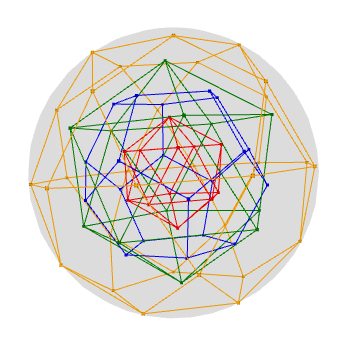
\includegraphics[width=\linewidth]{a5}
    \caption{$A_5$ illustrated in $\overline{B}$}
    \end{subfigure}
    \begin{subfigure}{.49\linewidth}
    \centering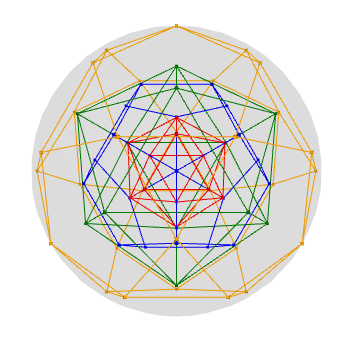
\includegraphics[width=\linewidth]{a5-3cycle}
    \caption{viewed along a 3-cycle axis}
    \end{subfigure}
    \begin{subfigure}{.49\linewidth}
    \centering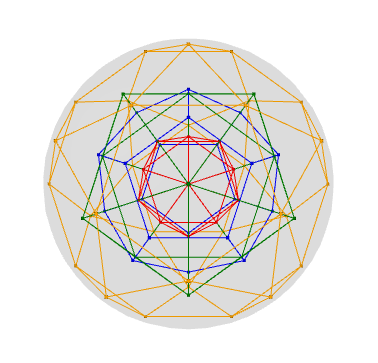
\includegraphics[width=\linewidth]{a5-5cycle}
    \caption{viewed along a 5-cycle axis}
    \end{subfigure}
    \begin{subfigure}{.49\linewidth}
    \centering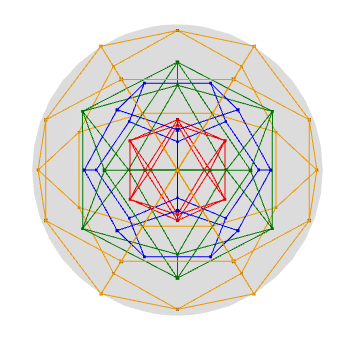
\includegraphics[width=\linewidth]{a5-2-2cycle}
    \caption{viewed along a 2-2-cycle axis}
    \end{subfigure}
    \caption{
        The conjugacy classes are color coded polyhedra \\\centering
        \begin{tabular}{c|c}
            red icosahedron & 5-cycles ($k=1$) \\
            blue dodecahedron & 3-cycles \\
            green icosahedron & 5-cycles ($k=2$) \\
            yellow icosidodecahedron & 2-2-cycles
        \end{tabular}
    }
    \label{fig:a5}
\end{figure}

Note that $A_4 = S_4^2=<(123), (12)(34)>\subset S_4$ is just the 3-cycles and the 2-2-cycles as:
\begin{itemize}
    \item 2-cycles and 2-2-cycles square to the identity
    \item 3-cycles are sent to 3-cycles, and 4-cycles to 2-2-cycles by squaring
\end{itemize}
Equivalently, the symmetries of a tetrahedron are a the cube and a half-octohedron, or a type or equilateral "triangle"; a geometric object with 3 vertices joined by equal length edges embedded in $SO(3)$, but there are 6 edges instead of 3: as each pair of vertices can be joined by an equal length pair of edges forming a great circle through the vertices and perpendicular to the great circles formed the same way through the other vertex.

This process works almost the exact same way for $A_5$ (fig. \ref{fig:a5}) as the symmetries of the dodecahedron with one important distinction due to 5-cycles splitting into two conjugacy classes. The class equation for $A_5$ is $1+12+20+12+15 = 5!/2$, and the two 12's come from the split 5-cycles which are permuted to each other via the one outer automorphism of $A_5$ by a 2-cycle in $S_5$. Said another way, this is because there are two possible values of $k$ for $n=5$ in Thm. \ref{thm:sphereclass}: $k=1,2$, corresponding to rotations by $2\pi/5$ and $4\pi/5$. The correspondence is as follows:
\begin{itemize}
    \item 3-cycles fix vertices of a dodecahedron and are order 3, so their representatives are a dodecahedron of radius $2\pi/3$.
    \item 5-cycles fix vertices of the dual icosahedron and are order 5, so their representatives are a \emph{pair} of dual icosahedra, one of radius $2\pi/5$ and one $4\pi/5$.
    \item 2-2-cycles fix vertices of the edge-midpoint dual\footnote{of both the dodecahedron and icosahedron} icosidodecahedron and are order 2, so their representatives are antipodal pairs of vertices of an icosidodecahedron of radius $\pi$.
\end{itemize}

\section{Conclusions}
The geometry of finite groups themselves is intimately related the geometry of objects whose symmetries are that group: element order and conjugacy class determine the placement of elements in our flattened view as a polyhedron of vertices embedded in a sphere of a certain radius. The relative orientation of distinct classes was determined by the geometric duality between the respective polyhedra. Using these tools we described visualizations of finite subgroups of $SO(3)$ without any explicit calculations.
%    Bibliographies can be prepared with BibTeX using amsplain,
%    amsalpha, or (for "historical" overviews) natbib style.
\bibliographystyle{amsplain}
%    Insert the bibliography data here.
\bibliography{references}

\end{document}